\section{Technical framework and experimental methodology}
\label{sec:framework}

\subsection{Parametric articulated representation}
\label{sec:representation}

The model has a fixed-topology template of $10{,}235$ vertices, a kinematic
tree of $55$ joints, per-vertex skinning weights, a $25$-dimensional shape
basis, a bilateral symmetry map and authored joint rotation limits. Fixed
topology is what makes correspondence meaningful: vertex $i$ denotes the same
anatomical locus in every fit, so a registered corpus lives in one coordinate
system. A shaped vertex $\bar{\mathbf v}_i(\bm\beta)=\mathbf v^{0}_i+\sum_k\beta_k\mathbf s_{ik}$
is posed by linear blend skinning,
\begin{equation}
\mathbf v_i(\bm\beta,\bm\theta)=\sum_{j=1}^{55} w_{ij}\,G_j(\bm\theta)\,\bar{\mathbf v}_i(\bm\beta),
\qquad G_j(\bm\theta)=\prod_{k\in\mathrm{anc}(j)}\big[R(\theta_k)\,|\,\mathbf t_k\big].
\label{eq:lbs}
\end{equation}
The latent variables form a hierarchy: $\bm\beta$ encodes morphology,
$\bm\theta$ articulation, $s$ (with per-joint scales) size, and $\mathbf d$ the
residual geometry that the shape space cannot express. The forward model maps
these variables to a surface, $V=S(\bm\beta,\bm\theta,s)+\mathbf d$; the
registration problem inverts this mapping from surface observations alone. Two
structural consequences recur. A rotation error at a proximal joint changes
$G_j$ for every descendant and so displaces everything distal to it; and the
surface depends on joint \emph{positions} only through $G_j$, so a surface can
look right while the skeleton inside it is wrong.

\subsection{Registration objective and identifiability}
\label{sec:objective}

Let $X$ and $Y$ be area-weighted point samples ($N=6000$ each) of the model
surface $V$ and of the scan $T$. The registration objective is
\begin{equation}
\mathcal L=\underbrace{w_{\mathrm{ch}}\mathcal L_{\mathrm{ch}}+w_{\mathrm n}\mathcal L_{\mathrm n}}_{\text{observe the target}}
+\underbrace{w_{\mathrm e}\mathcal L_{\mathrm e}+w_{\Delta}\mathcal L_{\Delta}+w_{\mathrm o}\mathcal L_{\mathrm o}}_{\text{regularise the mesh}}
+\underbrace{w_{\mathrm m}\mathcal L_{\mathrm m}+w_{\mathrm{sym}}\mathcal L_{\mathrm{sym}}+w_{\ell}\mathcal L_{\ell}+w_{\sigma}\mathcal L_{\sigma}}_{\text{priors on the model}},
\label{eq:objective}
\end{equation}
with the symmetric Chamfer term
$\mathcal L_{\mathrm{ch}}=\frac1N\sum_{x\in X}\min_{y\in Y}\|x-y\|^2+\frac1N\sum_{y\in Y}\min_{x\in X}\|x-y\|^2$,
the mean squared edge length $\mathcal L_{\mathrm e}$, the uniform Laplacian
$\mathcal L_{\Delta}$ and the deformation penalty
$\mathcal L_{\mathrm o}=\frac1{|V|}\sum_v\|\mathbf d_v\|^2$, the latter three in
the spirit of as-rigid-as-possible modelling~\cite{arap}. The model priors keep
the midsagittal vertex set on the symmetry plane ($\mathcal L_{\mathrm m}$), tie
left to right ($\mathcal L_{\mathrm{sym}}$), penalise joint rotations outside the
authored box with a hinge that is flat inside and linear outside
($\mathcal L_{\ell}$), and bound per-joint scale beyond a free band of a factor
two with $\mathcal L_{\sigma}=\operatorname{mean}\,(|\ln s_{jk}|-\ln 2)_+^2$, a
soft penalty by design so that no gradient discontinuity appears where
difficult specimens live. Table~\ref{tab:objective} states what each term
\emph{observes}, which is the information the optimiser actually has. What the
output additionally requires (joint location, anatomical identity,
within-structure correspondence) appears in no term. Two elementary properties
of Equation~\eqref{eq:objective} follow, and they organise every experiment
below.

\begin{table}[!htb]
\centering
\caption{Terms of the registration objective and what each one observes.}
\label{tab:objective}
\begin{tabular}{@{}L{0.26\linewidth}L{0.66\linewidth}@{}}
\toprule
\textbf{Term} & \textbf{What it observes}\\
\midrule
$\mathcal L_{\mathrm{ch}}$, $\mathcal L_{\mathrm n}$ & The scan as a point set with normals; a function of two
 surfaces, blind to which vertex is which\\
$\mathcal L_{\mathrm e}$, $\mathcal L_{\Delta}$, $\mathcal L_{\mathrm o}$ & Mesh regularity and size of the residual
 deformation; independent of the target\\
$\mathcal L_{\mathrm m}$, $\mathcal L_{\mathrm{sym}}$ & Bilateral consistency of the model\\
$\mathcal L_{\ell}$, $\mathcal L_{\sigma}$ & Joint \emph{angles} and per-joint scales against authored ranges\\
\bottomrule
\end{tabular}
\end{table}

\textbf{Label invariance of the data terms.} The target-dependent terms depend on
$V$ only through the point set and its normals. For any permutation $P$ of the
vertex index, $\mathcal L_{\mathrm{ch}}(PV,T)=\mathcal L_{\mathrm{ch}}(V,T)$: the
data cannot distinguish a solution from one that assigns the same surface to
different anatomical labels. Identity can therefore enter only through the
structure of the model's image (fixed topology, skinning, symmetry, limits), so
identifiability is a property of the \emph{model and its priors}, not of the
data term.

\textbf{Pose--deformation ambiguity.} Because the deformation is added after
skinning, any alternative pose $\bm\theta'$ reproduces exactly the same surface
with $\mathbf d'=\mathbf d+S(\bm\beta,\bm\theta,s)-S(\bm\beta,\bm\theta',s)$. The
data terms, and the edge and Laplacian terms, which also depend only on $V$, are
constant along this family, a gauge freedom of the parameterisation. Among the pose-dependent terms only the deformation
penalty $\mathcal L_{\mathrm o}$, the joint-limit hinge $\mathcal L_{\ell}$ and the
symmetry priors distinguish its members, so the pose estimate is
\begin{equation}
\hat{\bm\theta}=\arg\min_{\bm\theta'}\;w_{\mathrm o}\,\frac1{|V|}\big\|S(\bm\beta,\bm\theta,s)-S(\bm\beta,\bm\theta',s)+\mathbf d\big\|^2+w_{\ell}\mathcal L_{\ell}(\bm\theta')+\cdots,
\label{eq:gauge}
\end{equation}
that is, \emph{the pose that needs the least deformation}. This is a prior, not
an observation. It recovers the true pose exactly when the unmodelled part of the
scan is small relative to the displacement a pose error induces, which holds for
model-generated targets ($\mathbf d^\ast=0$) but is not guaranteed for real
specimens. Figure~\ref{fig:gauge} shows the consequence: as $w_{\mathrm o}$
decreases the objective along the family flattens, the pose becomes
underdetermined, and small contributions from other terms decide where the
optimiser stops. Reweighting a term that does not measure the missing quantity
cannot recover it.

\begin{figure}[!htb]
\centering
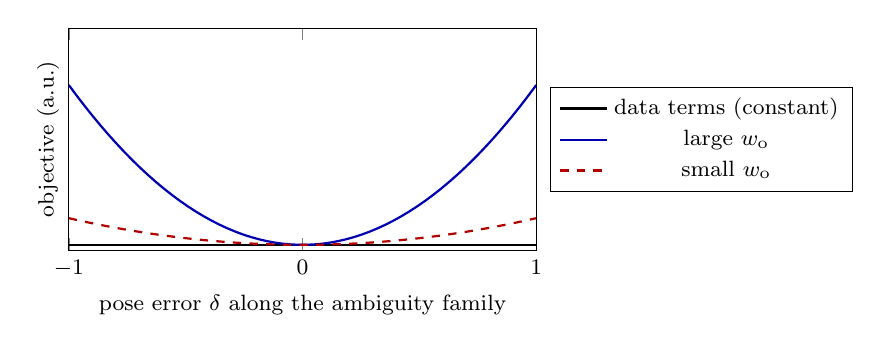
\begin{tikzpicture}
\begin{axis}[width=0.62\linewidth,height=4.4cm,xlabel={pose error $\delta$ along the ambiguity family},
 ylabel={objective (a.u.)},xlabel style={font=\footnotesize},ylabel style={font=\footnotesize},
 tick label style={font=\footnotesize},legend style={font=\footnotesize,at={(1.03,0.5)},anchor=west},
 domain=-1:1,samples=60,ymin=0,ymax=1.25,xmin=-1,xmax=1,xtick={-1,0,1},ytick=\empty]
\addplot[thick,black] {0.03};
\addplot[thick,blue!70!black] {0.9*x^2+0.03};
\addplot[thick,red!70!black,dashed] {0.15*x^2+0.03};
\legend{data terms (constant), large $w_{\mathrm o}$, small $w_{\mathrm o}$}
\end{axis}
\end{tikzpicture}
\caption[Pose--deformation ambiguity]{Schematic of Equation~\eqref{eq:gauge}.
Along the family of poses that reproduce the same surface, the data terms are
constant and only the deformation penalty (and the limits) vary. A large penalty
gives a well-conditioned minimum at the true pose ($\delta=0$); a small one
leaves a nearly flat valley in which the pose is set by whatever else differs
between candidates.}
\label{fig:gauge}
\end{figure}

\subsection{End-to-end fitting pipeline}
\label{sec:pipeline}

The pipeline (Figure~\ref{fig:pipeline}) has four stages: preprocessing,
initialisation, registration and, new in this work, a correspondence-audit
stage that reports how far each vertex's identity can be trusted rather than
only how close the surfaces are. The registration stage is organised to supply,
step by step, the information the objective lacks without adding an observation
of identity (Table~\ref{tab:stages}). Six identical legs make a global Chamfer
term multimodal, since any leg can be matched by any leg's surface, whereas the
body is three blobs on an axis and essentially unimodal. A body-only stage
therefore places the body and, with it, the six coxae; the target is then
partitioned by anatomical territory and each leg chain is fitted against only
its own assigned points; all joints are released with the partition kept; and
only then do the surface stages free pose, shape, scales and deformation
together, with the deformation penalty deliberately expensive so that deformation
absorbs species detail and not pose error. The partition supplies \emph{regional}
identity, not within-region location, which is why it removes the multimodality
and still leaves the problem analysed in Section~\ref{sec:oracle}.



\begin{figure}[!htb]
\centering
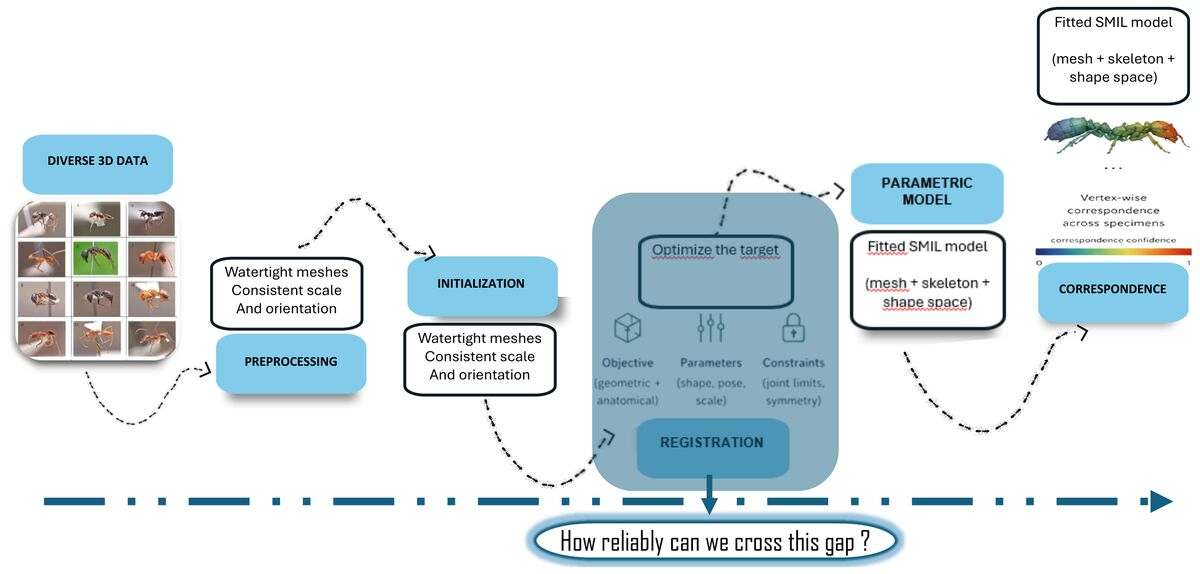
\includegraphics[width=0.9\linewidth]{figures/fig_pipeline_full.jpg}
\caption[The registration pipeline]{The registration pipeline, from diverse raw scans to a
fitted parametric model with vertex-wise correspondence. The correspondence stage did not
exist before this work.}
\label{fig:pipeline}
\end{figure}

\begin{table}[!htb]
\centering
\caption{Stages of the registration recipe.}
\label{tab:stages}
\begin{tabular}{@{}L{0.14\linewidth}L{0.25\linewidth}L{0.27\linewidth}L{0.25\linewidth}@{}}
\toprule
\textbf{Stage} & \textbf{Moves} & \textbf{Observes} & \textbf{Purpose}\\
\midrule
Body & Body chain; legs frozen & Global Chamfer & Place body and coxae\\
Legs & Leg chains; body frozen & Own-territory points per leg &
 Remove six-leg multimodality\\
Joints & All joints; partition kept & Partitioned Chamfer & Refine without
 cross-leg matching\\
Surface, coarse & Pose, shape, scales, $\mathbf d$ ($w_{\mathrm o}=5$) &
 Symmetric Chamfer, 6000 samples & Fit surface; deformation expensive\\
Surface, fine & Same, smaller steps ($w_{\mathrm o}=2$) & Chamfer weight halved,
 regularisers relaxed & Absorb residual detail\\
\bottomrule
\end{tabular}
\end{table}

\subsection{Synthetic correspondence benchmark}
\label{sec:synthetic}

The quantity of interest is not directly observed in an ordinary scan, so every claim
rests on one of two kinds of ground truth. The model can generate its own
targets: sample $(\bm\beta,\bm\theta)$, pose the template, export an anonymous
mesh (optionally degraded), refit it with the production fitter, and compare
fitted vertex $i$ with true vertex $i$. This gives exact correspondence error at
no annotation cost and permits one factor at a time to be varied. Because the
target comes from the model, the benchmark isolates the inverse problem from data
quality and gives a lower bound for real scans; correctness on real specimens is
established by the expert benchmark. The correspondence accuracy is
$A=\frac1{|V|}\sum_i\mathbb 1\big[\arg\min_k\|\hat v_i-v^\ast_k\|=i\big]$,
reported overall and per anatomical part (leg and segment accuracy). It is read
against its own ceiling: feeding the ground-truth mesh itself through the audit
scores below $1$ (about $0.99$ for legs and $0.97$ for segments) because points
near a segment boundary are ambiguous even under exact correspondence, so a gap
is measured to the ceiling and not to unity.

\subsection{Expert Joint Alignment Benchmark}
\label{sec:jab}

For real specimens, an expert placed 3D joints manually, and the Joint Alignment
Benchmark (JAB) was built on them: 11 specimens, 12 strategies, 3 optimiser seeds
and $396$ fits, pre-registered and frozen with a SHA-256 hash before any strategy
was run. Each strategy changes exactly one factor of the production recipe. The
joint error is $e_{sj}=\|\hat j_{sj}-j^\ast_{sj}\|/\mathrm{WL}_s$ in units of
Weber's length (WL, a posture-independent body-size measure), summarised per
specimen by the median over joints and averaged over seeds, with no post-hoc
alignment: Procrustes alignment spreads a few grossly misplaced joints over all
landmarks and masks global placement error~\cite{vonCramon}, and here it
increased the error on 9 of 11 specimens.

Because the reference annotation is itself part of the measurement system, its
coordinate convention was audited before any inference was made from it. Earlier
joint errors had been measured in a frame fitted \emph{to the production
skeleton}; a residual computed on the points used to define an alignment is a
fiducial-type error and says little about error elsewhere~\cite{fitzpatrick}.
Re-registering the annotations through each scan mesh (to a residual below
$10^{-7}$ of the diagonal) moved the measured production error from $42.7\%$ to
$25.1\%$ of WL without touching the fitter. The audit also corrected four
mirror-image annotation scenes, excluded one specimen annotated on another
specimen's mesh, and applied the axis map $(x,y,z)\mapsto(x,z,-y)$ to
surface-landmark coordinates stored in Blender's frame, so that analyses built on
the earlier surface landmarks were retired.

\subsection{Multi-level evaluation protocol}
\label{sec:protocol}

The central methodological challenge is that anatomical correspondence is not
directly observable. Three evidence levels are therefore always used together
(Table~\ref{tab:levels}), and an intervention is adopted only if it does not
degrade levels 1--2 and is checked at level 3 wherever ground truth exists.

\begin{table}[!htb]
\centering
\caption{The three evidence levels of the evaluation protocol.}
\label{tab:levels}
\begin{tabular}{@{}L{0.22\linewidth}L{0.40\linewidth}L{0.30\linewidth}@{}}
\toprule
\textbf{Level} & \textbf{Metrics} & \textbf{Question answered}\\
\midrule
1. Geometric agreement & Chamfer, F-score, per-part variants & Does the fitted
 surface cover the scan?\\
2. Structural integrity & Edge-length distortion, Laplacian and ARAP deviation,
 normal consistency & Was that agreement obtained by distorting the model?\\
3. Anatomical correctness & Synthetic vertex-identity error; expert joint
 error & Does model location $i$ correspond to the anatomical location it
 represents?\\
\bottomrule
\end{tabular}
\end{table}

\textbf{An adversarial test of the metric.} A metric that a targeted attack can
improve by damaging the reconstruction cannot be the sole judge of a fit.
Deliberately snapping distal vertices onto the nearest target surface improves a
per-part surface distance by $53\%$ while edge-length distortion rises $7.5$-fold:
the surface metric improves exactly as the geometric integrity collapses. This is
the clearest justification for the framework.

\textbf{Statistics.} The specimen is the unit of inference. Strategies are
compared with paired Hodges--Lehmann shifts and exact Wilcoxon-inverted intervals,
Holm-corrected across the 11 contrasts, and ranked with a Friedman test~\cite{demsar};
a joint-level mixed model with crossed specimen and joint effects accounts for
the nesting. A strategy is declared \emph{equivalent} to the reference when its
90\% confidence interval lies inside $\pm2.5\%$ of WL, the measured annotation
repeatability, which is the interval-inclusion form of two one-sided tests at
$\alpha=0.05$~\cite{lakens}. At $n=11$ the pre-registered specimen-level test
resolves effects that are consistent across about ten of eleven specimens; smaller
effects are carried by their intervals and by the mixed model.
